\documentclass[border=4pt]{standalone}
% shared style for all PyTBA topology diagrams (\input by each standalone file)
\usepackage{mathpazo}
\usepackage{amsmath}
\usepackage{tikz}
\usetikzlibrary{positioning,arrows.meta,calc,decorations.pathreplacing,fit,backgrounds}
\tikzset{
  host/.style={draw=blue!55!black, fill=blue!7, rounded corners=2pt, align=center,
               minimum height=9mm, minimum width=22mm, font=\small},
  blk/.style={draw=black!60, fill=black!4, rounded corners=2pt, align=center,
              minimum height=8mm, font=\small},
  chan/.style={draw=orange!70!black, fill=orange!8, rounded corners=2pt, align=center,
               minimum height=9mm, font=\small},
  lossbox/.style={draw=red!70!black, fill=red!6, rounded corners=2pt, align=center, font=\footnotesize},
  data/.style={-{Stealth[length=2.2mm]}, thick},
  ack/.style={-{Stealth[length=2mm]}, dashed, black!60},
  lbl/.style={font=\footnotesize, align=center},
  brace/.style={decorate, decoration={brace, amplitude=4pt}, thick, black!70},
}

\begin{document}
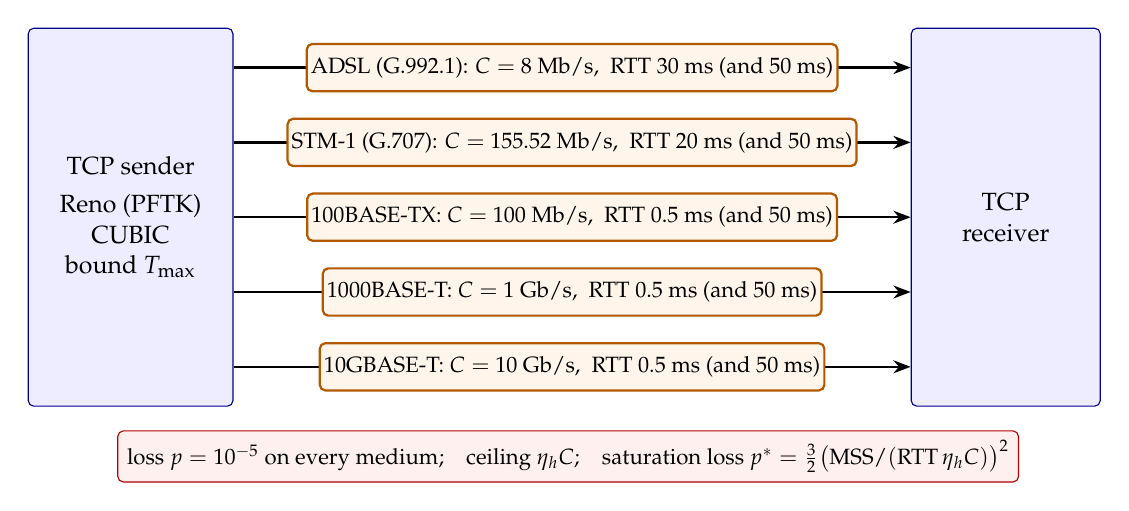
\begin{tikzpicture}
\node[host, minimum height=48mm, minimum width=26mm] (s) {TCP sender\\[1mm]Reno (PFTK)\\CUBIC\\bound $T_{\max}$};
\node[host, minimum height=48mm, minimum width=24mm, right=86mm of s] (r) {TCP\\receiver};
\foreach \i/\name/\rate/\rtt in {1/{ADSL (G.992.1)}/{8 Mb/s}/{30 ms}, 2/{STM-1 (G.707)}/{155.52 Mb/s}/{20 ms},
     3/{100BASE-TX}/{100 Mb/s}/{0.5 ms}, 4/{1000BASE-T}/{1 Gb/s}/{0.5 ms}, 5/{10GBASE-T}/{10 Gb/s}/{0.5 ms}} {
  \pgfmathsetmacro{\y}{19-9.5*(\i-1)}
  \draw[data] ($(s.east)+(0,\y mm)$) -- node[chan, minimum height=6mm, inner sep=1.5pt, font=\footnotesize]
     {\name: $C=$ \rate,\ \ RTT \rtt\ (and 50 ms)} ($(r.west)+(0,\y mm)$);
}
\node[lossbox, below=3mm of $(s.south)!0.5!(r.south)$] {loss $p=10^{-5}$ on every medium;\quad
  ceiling $\eta_h C$;\quad saturation loss $p^*=\tfrac{3}{2}\big(\mathrm{MSS}/(\mathrm{RTT}\,\eta_h C)\big)^2$};
\end{tikzpicture}
\end{document}
